\documentclass[12pt]{beamer}
\usepackage{listings}
\usepackage[]{color}
%\usepackage{bbding}
%\usepackage{ragged2e}
\usepackage{tikz}
\usetikzlibrary{decorations.pathreplacing}
\usetikzlibrary{calc}

\beamertemplatenavigationsymbolsempty
\AtBeginSection[]
{
    \begin{frame}
    \frametitle{Table of Contents}
    \tableofcontents[currentsection]
    \end{frame}
}
\setlength{\tabcolsep}{10pt}
\newcommand{\bigoh}[1]{\mathcal{O}\left(#1\right)}
\newcommand{\TLE}{\textcolor{blue}{TLE}}
\newcommand{\WA}{\textcolor{red}{WA}}
\newcommand{\MLE}{\textcolor{orange}{MLE}}
\newcommand{\AC}{\textcolor{green}{AC}}
\newcommand{\blank}{\vspace{.5cm}}

\definecolor{mygreen}{rgb}{0,0.6,0}
\definecolor{mygray}{rgb}{0.5,0.5,0.5}
\definecolor{mymauve}{rgb}{0.58,0,0.82}

\lstset{ %
  backgroundcolor=\color{white},   % choose the background color; you must add \usepackage{color} or \usepackage{xcolor}
  basicstyle=\tiny,        % the size of the fonts that are used for the code
  breakatwhitespace=false,         % sets if automatic breaks should only happen at whitespace
  breaklines=true,                 % sets automatic line breaking
  commentstyle=\color{mygreen},    % comment style
  deletekeywords={...},            % if you want to delete keywords from the given language
  escapeinside={\%*}{*)},          % if you want to add LaTeX within your code
  extendedchars=true,              % lets you use non-ASCII characters; for 8-bits encodings only, does not work with UTF-8
  frame=single,                    % adds a frame around the code
  keepspaces=true,                 % keeps spaces in text, useful for keeping indentation of code (possibly needs columns=flexible)
  keywordstyle=\color{blue},       % keyword style
  language=C++,                 % the language of the code
  morekeywords={*,...},            % if you want to add more keywords to the set
  numbers=left,                    % where to put the line-numbers; possible values are (none, left, right)
  numbersep=5pt,                   % how far the line-numbers are from the code
  numberstyle=\tiny\color{mygray}, % the style that is used for the line-numbers
  rulecolor=\color{black},         % if not set, the frame-color may be changed on line-breaks within not-black text (e.g. comments (green here))
  showspaces=false,                % show spaces everywhere adding particular underscores; it overrides 'showstringspaces'
  showstringspaces=false,          % underline spaces within strings only
  showtabs=false,                  % show tabs within strings adding particular underscores
  stepnumber=1,                    % the step between two line-numbers. If it's 1, each line will be numbered
  stringstyle=\color{mymauve},     % string literal style
  tabsize=2                      % sets default tabsize to 2 spaces
}

\title{Binary Search}
\subtitle{}
\author{beOI Training}
\institute{\includegraphics[height=12em]{../share/beoi-logo}}

\begin{document}

\frame{\titlepage}

\section{Basic algorithm}

\begin{frame}
    \frametitle{Why do we need it?}
    \textbf{Searching a sorted list}: \\\blank
    Given a sorted array $A$, find the index of an element $v$ in this array.\\\blank
    
\end{frame}

\begin{frame}
	\frametitle{The algorithm}
    Look at the middle element and compare it with the number you're looking for. \\Is it:
    \begin{itemize}
    	\item{The same $\rightarrow$ Congratulations! }
    	\item{Smaller  $\rightarrow$ It can only be after this element}
    	\item{Bigger   $\rightarrow$ It can only be before this element}
    	
    \end{itemize}
    Repeat!\\\blank
    This is a divide-and-conquer algorithm
\end{frame}

\begin{frame}
	\frametitle{An example}
	\begin{center}
		$A = $
		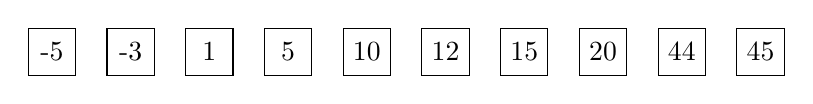
\begin{tikzpicture}
    	\coordinate (s) at (0,0);
    	\foreach \num in {-5,-3,1,5,10,12,15,20,44,45}{
      		\node[minimum size=6mm, draw, rectangle] at (s) {\num};
      		\coordinate (s) at ($(s) + (1,0)$);
   		} 
  		\end{tikzpicture}\\
		$v = 12$\\\blank
	\end{center}
	$low = 0$\\
	$high = 9$\\
	$mid = 4$

\end{frame}

\begin{frame}
	\frametitle{An example}
	\begin{center}
		$A = $
		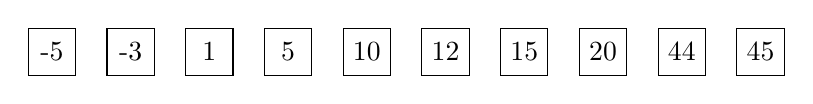
\begin{tikzpicture}
    	\coordinate (s) at (0,0);
    	\foreach \num in {-5,-3,1,5,10,12,15,20,44,45}{
      		\node[minimum size=6mm, draw, rectangle] at (s) {\num};
      		\coordinate (s) at ($(s) + (1,0)$);
   		} 
  		\end{tikzpicture}\\
		$v = 12$\\\blank
	\end{center}
	$low = 0$\\
	$high = 9$\\
	$mid = 4$

\end{frame}

\begin{frame}
	\frametitle{An example}
	\begin{center}
		$A = $
		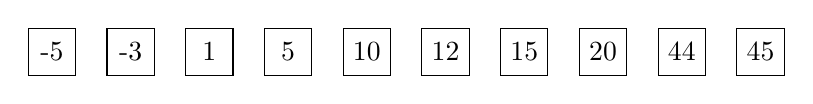
\begin{tikzpicture}
    	\coordinate (s) at (0,0);
    	\foreach \num in {-5,-3,1,5,10,12,15,20,44,45}{
      		\node[minimum size=6mm, draw, rectangle] at (s) {\num};
      		\coordinate (s) at ($(s) + (1,0)$);
   		} 
  		\end{tikzpicture}\\
		$v = 12$\\\blank
	\end{center}
	$low = 5$\\
	$high = 9$\\
	$mid = 7$

\end{frame}

\begin{frame}
	\frametitle{An example}
	\begin{center}
		$A = $
		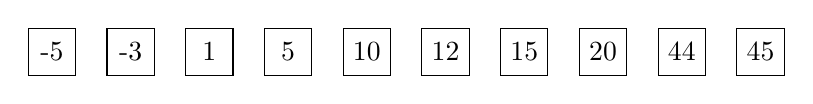
\begin{tikzpicture}
    	\coordinate (s) at (0,0);
    	\foreach \num in {-5,-3,1,5,10,12,15,20,44,45}{
      		\node[minimum size=6mm, draw, rectangle] at (s) {\num};
      		\coordinate (s) at ($(s) + (1,0)$);
   		} 
  		\end{tikzpicture}\\
		$v = 12$\\\blank
	\end{center}
	$low = 5$\\
	$high = 6$\\
	$mid = 5$\\
	\begin{center}
		\includegraphics[scale=0.3]{img/psi.jpg}
	\end{center}

\end{frame}

\begin{frame}
	\frametitle{What if it's not there?}
	We just stop when there's no more items to consider $\rightarrow low > high$
\end{frame}

\begin{frame}
	\frametitle{The code}
	\lstinputlisting{listings/binary-search.cpp} \pause \blank
	Complexity? $\bigoh{log(n)}$
\end{frame}

\begin{frame}
	\frametitle{The devil's in the details}
	Beware for off-by-one errors when changing boundaries!\\
	How to handle duplicate values?\\
	Watch out for overflow when computing indices.
	\begin{center}
		\includegraphics[scale=0.2]{img/caution.jpg}
	\end{center}
\end{frame}
\section{Other applications}
\begin{frame}
	\frametitle{So...just searching?}
	Yep, that's it!\pause\\
	Well, not only in an array.\pause\\
	Only condition: static sorted \textit{sequence}
\end{frame}

\begin{frame}
	\frametitle{Bisection method}
	Find a hard root of a function.\\
	Binary search on real numbers. \\
	Example: $x^3 - 4x - 9 = 0$
\end{frame}

\begin{frame}
	\frametitle{The code: iterative}
	\lstinputlisting{listings/bisection.cpp}
\end{frame}

\begin{frame}
	\frametitle{The code: recursive}
	\lstinputlisting{listings/bisection-rec.cpp}
\end{frame}

\begin{frame}
	\frametitle{Binary search the answer: possibility 1}
	You don't know how to find the answer directly.\\
	BUT: you do know how to check how close you are. \\
	\begin{center}
		\includegraphics[scale=0.3]{img/catrescue.jpg}
	\end{center}
\end{frame}

\begin{frame}
	\frametitle{Binary search the answer: possibility 2}
	You don't know how to find the answer directly.\\
	BUT: you do know how to check if it's possible. \\
	\begin{center}
		\includegraphics[scale=0.3]{img/catrescue.jpg}
	\end{center}
	$A = $
		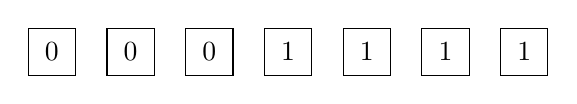
\begin{tikzpicture}
    	\coordinate (s) at (0,0);
    	\foreach \num in {0,0,0,1,1,1,1}{
      		\node[minimum size=6mm, draw, rectangle] at (s) {\num};
      		\coordinate (s) at ($(s) + (1,0)$);
   		} 
  		\end{tikzpicture}\\
\end{frame}

\section{Exercises}

\begin{frame}
	\frametitle{Exercises}
	\begin{itemize}
		\item Code a binary search!
		\item UVA 11057
		\item UVA 10567
		\item (UVA 957)
		\\\blank
		\item UVA 10341
		\item UVA 11413
		\item UVA 11935
		\\\blank
		\item UVA 12190 (very tedious!)
	\end{itemize}
	
\end{frame}

\end{document}
